\appendix

\chapter{Modelos adicionales Ecore}
\label{appendix:modelos_ecore_tree}

En esta sección anexa aparecen las figuras que por ocupar demasiado tamaño, no proceden aparecer en el contenido principal de la memoria.

\begin{landscape}

\begin{figure}
	\centering
    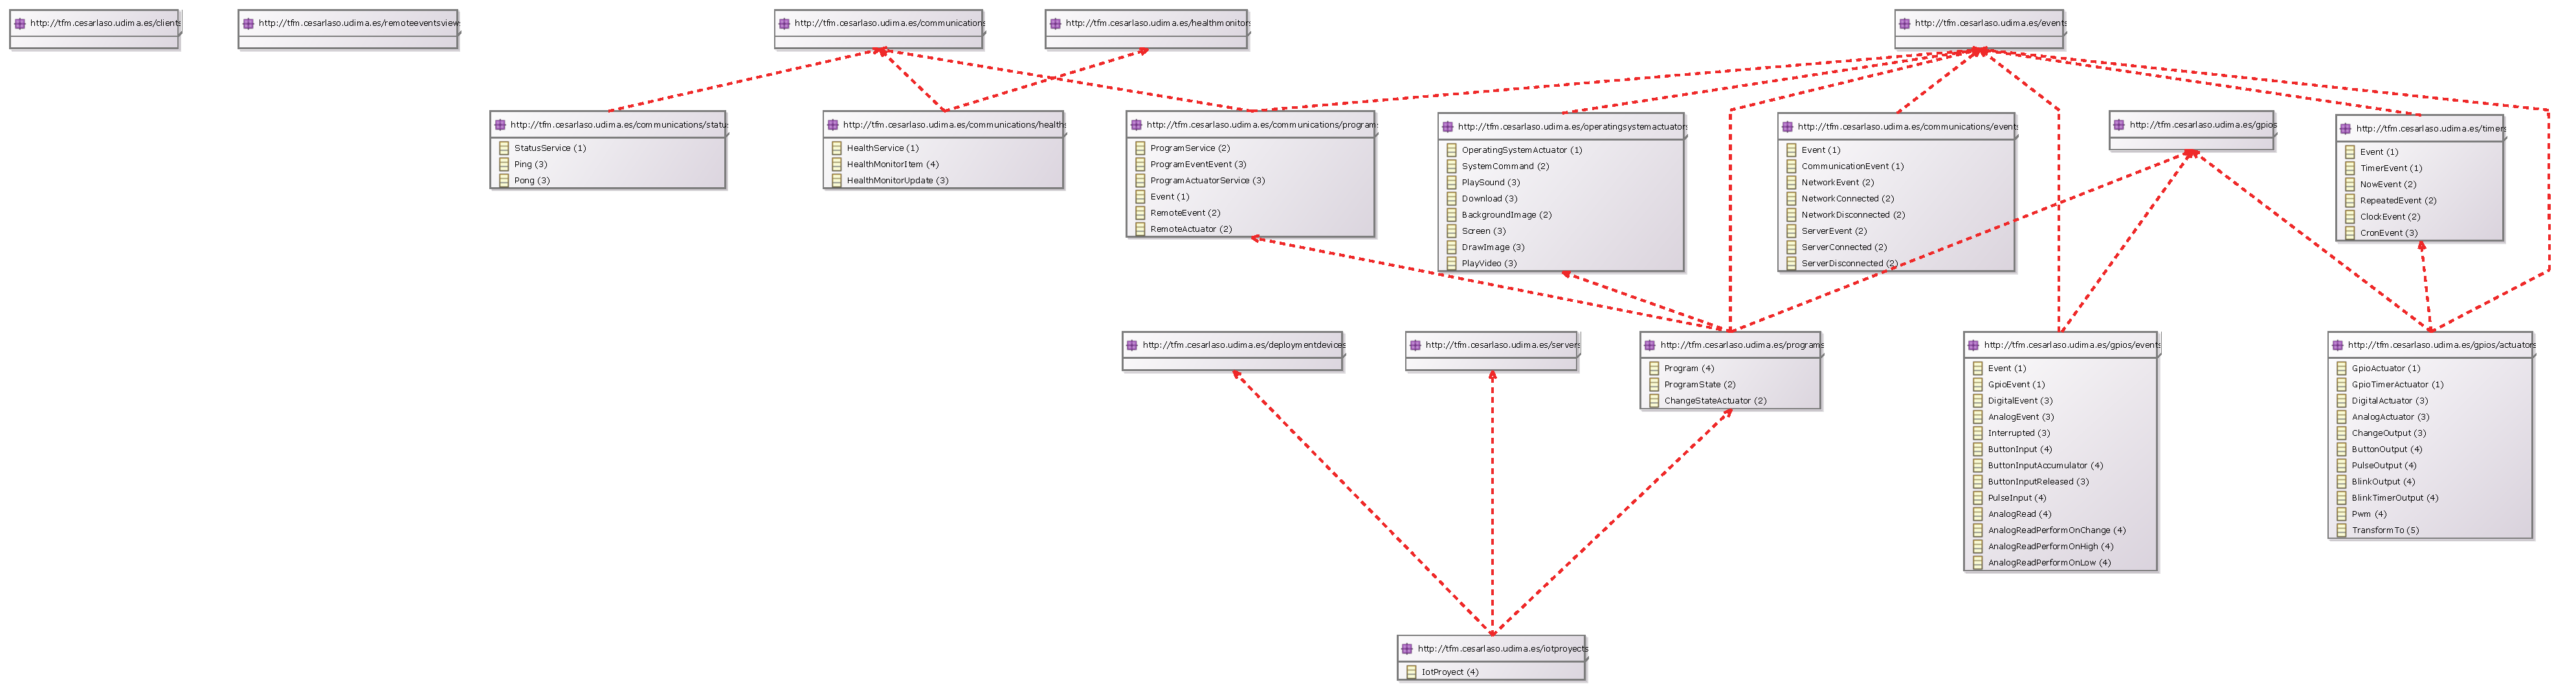
\includegraphics[width=\textwidth]{images/models/iotproyects_package_dependencies.pdf}
    \sourcepropia{}
    \caption{Proyecto IOT - Representación de las dependencias entre los modelos}
    \label{fig:modelo_iotpackages}
\end{figure}

\begin{figure}
\centering
    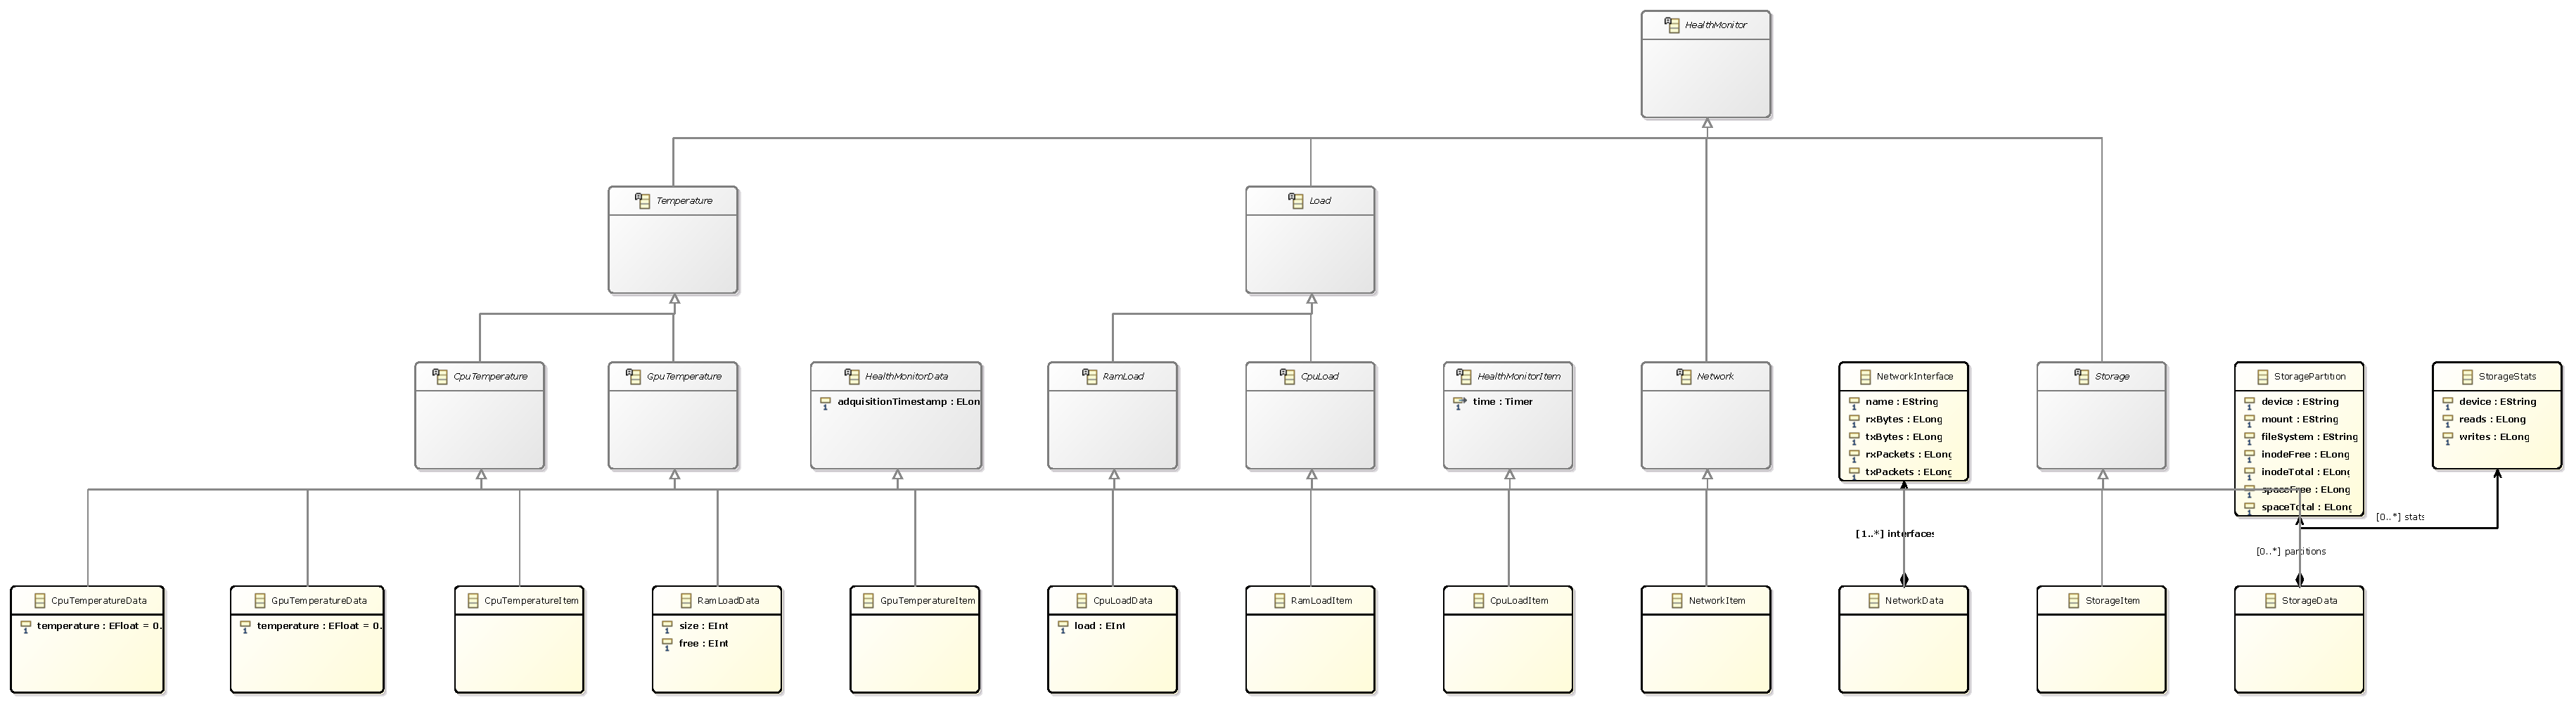
\includegraphics[width=\textwidth]{images/models/healthmonitors_class_diagram.pdf}
	\captionmodeloclase{Estado de salud}
	\label{fig:modelo_iot_health_classes}
\end{figure}

\begin{figure}
	\centering
    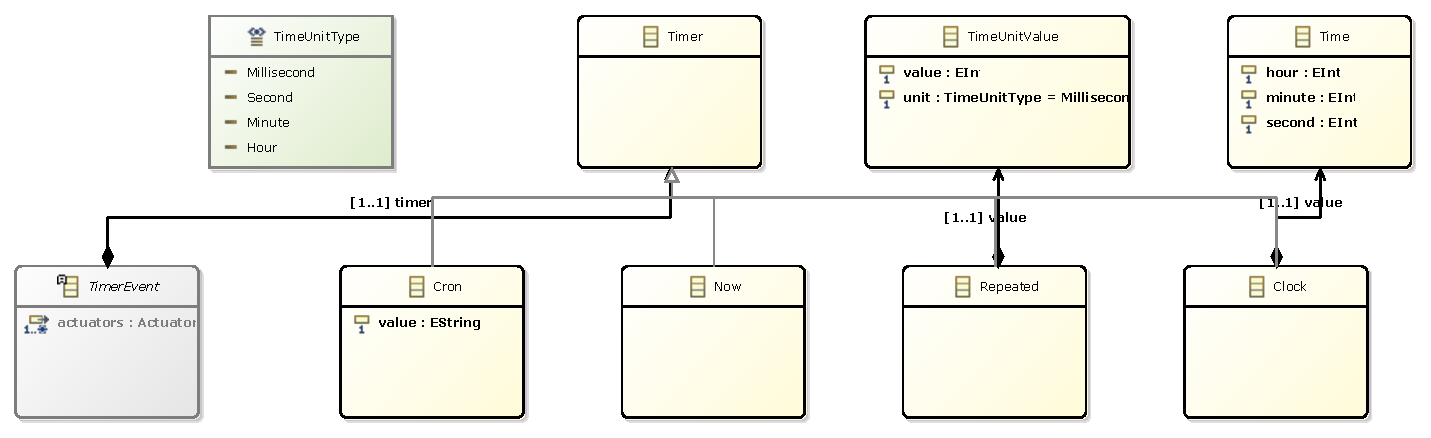
\includegraphics[width=\textwidth]{images/models/timers_class_diagram.pdf}
    \captionmodeloclase{Timers}
    \label{fig:modelo_timers_classes}
\end{figure}

\end{landscape}



\chapter{DSL}

\section{Ejemplo de programa ejemplo - Versión conceptual}
\label{appendix:dsl_motivacion_ejemplo}
\lstinputlisting{ejemplos/dsl_motivacion_ejemplo.txt}

\section{Gramática con el DSL del proyecto}
\label{appendix:dsl_final}
\lstinputlisting{ejemplos/Dsl.xtext}

\section{Xtend lectura de la gramática DSL mediante ecore y posterior conversión del modulo de comunicaciones, apartado telemetría a su implementación en Java}
\label{appendix:xtend_telemetry}
\lstinputlisting{ejemplos/telemetry_generator.xtend}




\chapter{Casos de uso - Ejemplos de programas escritos en el lenguaje creado}

\section{Programa adaptación maquinas con monedero electrónico a su versión conectada a internet}
\label{appendix:ejemplo_dsl_monedero}

Un simple dispositivo para tener control de las monedas que entran en un 
monedero de pulsos (cada moneda envía una anchura de pulso según su valor).
Con este programa conseguimos poder tener una contabilidad de cuanto esta generando cada máquina
de forma remota, almacenando en un servidor la fecha y hora de entrada de moneda en cada 
dispositivo.
Permite de forma remota simular la entrada de moneda, permitiendo poder pagar en el dispositivo
desde cualquier plataforma externa (por ejemplo móvil)

\lstinputlisting{ejemplos/ejemplo_dsl_1.iotproyect}



\section{Programa modernización futbolín}
\label{appendix:ejemplo_dsl_futbolin}

Este ejemplo esta basado en un proyecto real, en conjunto con un cliente fabricante de futbolines

El proyecto consistía en un dispositivo \gls{iot}. Su primera versión distribuida en Raspberry PI, posteriormente se reescribió a una versión más económica para el módulo ESP8266. En este caso, el uso de un \gls{dsl} hubiera permitido mantener los modelos en ámbas versiones. El dispositivo conectaba un futbolín con un sistema de gestión remota vía web de
administración  con las funcionalidades de alarmas, contabilidad, incidencias y junto a una aplicación para realizar torneos online entre jugadores para la plataforma Android.

Este ejemplo intenta emular un esqueleto de lo que podría ser la parte del proyecto \gls{iot} y su comunicación con un servidor.

\lstinputlisting{ejemplos/ejemplo_dsl_2.iotproyect}



\section{Programa modernización ascensor de hotel sin pantalla gráfica}
\label{appendix:ejemplo_dsl_ascensor}

Ejemplo de \gls{iot} conectado a un ascensor de un hotel.
Utilizado para modernizar un ascensor antiguo sin modificar nada del sistema del ascensor original, simplemente leyendo las salidas generadas por el sistema.

Este ejemplo está basado en un estudio de proyecto que realizamos para la adaptación de ascensores sin pantalla gráfica a una adaptación a pantalla con visualización, desarrollando un prototipo en Raspberry PI.

El sistema muestra las señales recibidas por el dispositivo electrónico del panel del ascensor en un pantalla gráfica.
La implementación corre mediante comandos que llaman al interfaz gráfico X-Window, mostrando imágenes y vídeos según la planta en la que se encuentre o eventos de tiempo determinados.  

\lstinputlisting{ejemplos/ejemplo_dsl_3.iotproyect}
